% Valentino Vranic
% Metody inzinierskej prace 2012/13

\documentclass{beamer}

%\usetheme{Warsaw}
\usetheme{Antibes}
%\usetheme{JuanLesPins}
%\usetheme{Goettingen}

%\usecolortheme{seahorse}
\usecolortheme{dolphin}
%\usecolortheme{rose}
% http://deic.uab.es/~iblanes/beamer_gallery/index_by_color.html
%\usecolortheme{beaver}

%\useoutertheme[]{sidebar}

\setbeamercovered{transparent}

\usepackage[slovak]{babel}
\usepackage[T1]{fontenc}
\usepackage[utf8]{inputenc}
\usepackage{url}

\usepackage{listings}

\lstset{language=C++,basicstyle=\fontsize{8}{9.6}\selectfont,showstringspaces=false,columns=fullflexible,identifierstyle=\ttfamily,keywordstyle=\bfseries,showstringspaces=false,columns=fullflexible}
%\lstset{language=C,basicstyle=\fontsize{10.5}{12.6}\selectfont,identifierstyle=\ttfamily,keywordstyle=\bfseries,showstringspaces=false,columns=fixed}

\def\BibTeX{\textsc{Bib}\kern-.08em\TeX} 

\newcommand{\footcite}[1]{\footnote{\tiny #1}}
\newcommand{\umlet}{.5}
\newcommand{\emp}[1]{\textit{\alert{#1}}}
\newcommand{\kw}[1]{\mbox{\textbf{#1}}}
\newcommand{\id}[1]{\texttt{#1}}
\newcommand{\stl}{\guillemotleft}
\newcommand{\str}{\guillemotright}

\newcommand{\lsti}{\lstinline[basicstyle=\fontsize{10.5}{12.1}\selectfont]}

\newcommand{\ssection}[1]{
	\section{#1}
	\begin{frame}[fragile=singleslide]\frametitle{}
	\Huge #1
	\end{frame}
}

\newcommand{\ssectionn}[1]{
	\section*{#1}
	\begin{frame}[fragile=singleslide]\frametitle{}
	\Huge #1
	\end{frame}
}

\newenvironment{program}{\begin{beamercolorbox}[rounded=true,shadow=true]{block body}\vspace{-4mm}}{\vspace{-2mm}\end{beamercolorbox}}

\setbeamercolor{fvystup}{fg=white,bg=black}
\newenvironment{vystup}{\begin{beamercolorbox}[rounded=true,shadow=true]{fvystup}}{\end{beamercolorbox}}

\newenvironment{poznamka}{\begin{beamercolorbox}[rounded=true,shadow=false]{block body}}{\end{beamercolorbox}}

\setbeamertemplate{footline}[page number]
{
%\insertpagenumber
%\begin{beamercolorbox}{section in head/foot}
%\vskip2pt\insertnavigation{\paperwidth}\vskip2pt
%\end{beamercolorbox}%
}



\author{Nikol Maljarová}
%\url{www.fiit.stuba.sk/~vranic}, \url{vranic@fiit.stuba.sk}}
%{\tiny \url{www.fiit.stuba.sk/~vranic}, \url{vranic@fiit.stuba.sk}}
\institute{
	Ústav informatiky, informačných systémov a softvérového inžinierstva\\
	Fakulta informatiky a informačných technológií\\
	Slovenská technická univerzita v Bratislave}

\subtitle{\vspace{3mm} Metódy inžinierskej práce 2023/2024}

\title{Sémantické vyhľadávanie
}

\date{\footnotesize 7. november 2023}




\begin{document}

\begin{frame}[fragile=singleslide]
\titlepage
\end{frame}


\begin{frame}[fragile=singleslide]\frametitle{O čom to je}
Ešte pre prehľadom prezentácie sa zvyčajne uvádza motivácia.

Bežne sa aj tu používajú odrážky, ale tento text je naschvál uvedený bez odrážok. Niekedy môže byť potrebné uviesť aj citáty\ldots{}

Toto je len príklad slajdov. Ako urobiť dobrú prezentáciu bolo vysvetlené na prednáške.
\end{frame}


\begin{frame}[fragile=singleslide]\frametitle{Prehľad}
\tableofcontents
\end{frame}


\section{Základné princípy}
% príkaz \ssection by vytvoril zvláštný slajd s názvom časti - v krátkych prezentáciách to prekáža, lebo oberá o čas

\begin{frame}[fragile=singleslide]\frametitle{Sémantické vs lexikálne vyhľadávanie}
\begin{itemize}
\item lexikálne - počet slov v dokumentoch
\item sémantické:
	\begin{itemize}
	\item význam slova
	\item vzťah k iným slovám
	\item vzťah ku téme dokumentu
	\end{itemize}
\item +: precíznejšie, inteligentnejšie
\item -: menej populárne - nedostatok stránok
\end{itemize}
\end{frame}

\section{Architektúra vyhľadávania}

\begin{frame}[fragile=singleslide]\frametitle{Štruktúra}
\begin{itemize}
\item všeobecná schéma:
	\begin{itemize}
	\item web crawling
	\item integrácia dát
	\item tvorenie ontológie
	\item metódy hľadania
	\item funkcie vyhľadávača
	\item zobrazenie výsledku
	\end{itemize}
\end{itemize}
\end{frame}

\section{Ontológia}
\begin{frame}[fragile=singleslide]\frametitle{Pojmy}
\begin{itemize}
\item Ontológia
\item Značkovanie
\end{itemize}
\end{frame}

\section{Typy vyhľadávania}

\section{Metódy vyhľadávania}

\begin{frame}[fragile=singleslide]\frametitle{Latentné sémantické indexovania}
\begin{itemize}
\item metóda Singular value decomposition
\item dokumenty a pojmy zobrazené ako vektory v priestore:
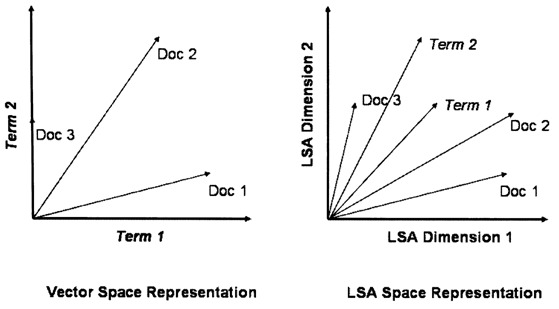
\includegraphics[scale=.35]{lsivektory.jpg}
\end{itemize}
\end{frame}

\section{Problémy}

\begin{frame}[fragile=singleslide]\frametitle{Ďalší slajd}
\begin{itemize}
\item Nejaký text
\item Ďalší text -- \emph{zvýraznený text}
\item \emp{Kľúčová poznámka} % príkaz definovaný v preambule

% odrážka s odkazom na zdroj:
\item Bol použitý balík beamer\footcite{\url{http://www.tex.ac.uk/tex-archive/macros/latex/contrib/beamer/doc/beameruserguide.pdf}}
\end{itemize}
\end{frame}


\begin{frame}[fragile=singleslide]\frametitle{Slajd len s obrázkom}
%\includegraphics[scale=.35]{diagram.pdf}
% pridajte vlastný obrázok a zrušte znák % pred príkazom \includegraphics vo formáte PDF prípadne PNG alebo JPG
% scale určuje veľkosť obrázku

{\tiny Nejaká poznámka k obrázku, možno zdroj\ldots}
\end{frame}


\begin{frame}[fragile=singleslide]\frametitle{Zvýraznenie syntaxe}
\begin{itemize}
\item Na zvýraznenie syntaxe stačí použiť balík listings so správne nastaveným programovacím jazykom
\begin{lstlisting}
int na_druhu(int i) {
   return i * i;
}

int main() {
   printf("%d", na_druhu(118));
   return 0;
}
\end{lstlisting}

\item Jazyk C++ je ešte zaujímavejší: je multiparadigmový\footcite{\url{J. O. Coplien. Multi-Paradigm Design for C++. Addison-Wesley, 1998.}}
\end{itemize}
\end{frame}


\begin{frame}[fragile=singleslide]\frametitle{Rámiky}
\begin{poznamka}
Text možno uviesť v rámiku
\end{poznamka}

\begin{itemize}
\item Program

\begin{program}
\begin{lstlisting}
void main() {
   printf("%d", na_druhu(118));
}

void na_druhu(int i) {
   return i * i;
}
\end{lstlisting}
\end{program}

\item Výstup
\begin{vystup}
\begin{lstlisting}
13924
\end{lstlisting}
\end{vystup}

\end{itemize}
\end{frame}



\section*{Zhodnotenie a ďalšia práca}
% hviezdička zabezpečí, aby sa táto časť neocitla v prehľade prezentácie - každá prezentácia má zhodnotenie a prehľad by sa tým zbytočne zahlcoval

\begin{frame}[fragile=singleslide]\frametitle{Zhodnotenie a ďalšia práca}
\begin{itemize}
\item Každá prezentácia musí byť nejako uzavretá
\item Ale vždy je čo robiť ďalej\ldots{}
\end{itemize}
\end{frame}


\end{document}




Text \end{document} za príkazom \end{document} LaTeX ignoruje, takže tu môžete odkladať veci (aj celé slajdy), ktoré nechcete vymazať, lebo ich ešte možno budete potrebovať, avšak ich v danom momente nechcete mať v slajdoch.
